
%% bare_conf.tex
%% V1.3
%% 2007/01/11
%% by Michael Shell
%% See:
%% http://www.michaelshell.org/
%% for current contact information.
%%
%% This is a skeleton file demonstrating the use of IEEEtran.cls
%% (requires IEEEtran.cls version 1.7 or later) with an IEEE conference paper.
%%
%% Support sites:
%% http://www.michaelshell.org/tex/ieeetran/
%% http://www.ctan.org/tex-archive/macros/latex/contrib/IEEEtran/
%% and
%% http://www.ieee.org/

%%*************************************************************************
%% Legal Notice:
%% This code is offered as-is without any warranty either expressed or
%% implied; without even the implied warranty of MERCHANTABILITY or
%% FITNESS FOR A PARTICULAR PURPOSE! 
%% User assumes all risk.
%% In no event shall IEEE or any contributor to this code be liable for
%% any damages or losses, including, but not limited to, incidental,
%% consequential, or any other damages, resulting from the use or misuse
%% of any information contained here.
%%
%% All comments are the opinions of their respective authors and are not
%% necessarily endorsed by the IEEE.
%%
%% This work is distributed under the LaTeX Project Public License (LPPL)
%% ( http://www.latex-project.org/ ) version 1.3, and may be freely used,
%% distributed and modified. A copy of the LPPL, version 1.3, is included
%% in the base LaTeX documentation of all distributions of LaTeX released
%% 2003/12/01 or later.
%% Retain all contribution notices and credits.
%% ** Modified files should be clearly indicated as such, including  **
%% ** renaming them and changing author support contact information. **
%%
%% File list of work: IEEEtran.cls, IEEEtran_HOWTO.pdf, bare_adv.tex,
%%                    bare_conf.tex, bare_jrnl.tex, bare_jrnl_compsoc.tex
%%*************************************************************************

% *** Authors should verify (and, if needed, correct) their LaTeX system  ***
% *** with the testflow diagnostic prior to trusting their LaTeX platform ***
% *** with production work. IEEE's font choices can trigger bugs that do  ***
% *** not appear when using other class files.                            ***
% The testflow support page is at:
% http://www.michaelshell.org/tex/testflow/



% Note that the a4paper option is mainly intended so that authors in
% countries using A4 can easily print to A4 and see how their papers will
% look in print - the typesetting of the document will not typically be
% affected with changes in paper size (but the bottom and side margins will).
% Use the testflow package mentioned above to verify correct handling of
% both paper sizes by the user's LaTeX system.
%
% Also note that the "draftcls" or "draftclsnofoot", not "draft", option
% should be used if it is desired that the figures are to be displayed in
% draft mode.
%
\documentclass[conference]{IEEEtran}
% Add the compsoc option for Computer Society conferences.
%
% If IEEEtran.cls has not been installed into the LaTeX system files,
% manually specify the path to it like:
% \documentclass[conference]{../sty/IEEEtran}

\usepackage{pdfsync}
\usepackage{comment}
\usepackage{amsmath}
\usepackage{amssymb}
\usepackage{amsthm}
\usepackage{calc}
\usepackage{color}
\usepackage{graphicx}
\usepackage{url}
\usepackage{xspace}
\usepackage{tikz}
\usepackage{pgfplots}
\usepackage{caption}
\usepackage{subcaption}

\usepackage[algo2e, noend, noline, linesnumbered]{algorithm2e}
\DontPrintSemicolon

\makeatletter
\newcommand{\pushline}{\Indp}% Indent
\newcommand{\popline}{\Indm}
\makeatother
\DeclareMathOperator{\pess}{pess}
\DeclareMathOperator{\opti}{opti}
\newcommand{\argmax}{\operatornamewithlimits{argmax}}

\captionsetup{compatibility=false}


%\usepackage{subfig}


% the note center!
%\newcommand{\marcl}[1]{\textbf{\color{red} #1 -- ML}}
%\newcommand{\rgg}[1]{\textbf{\color{red} #1 -- RG}}
\definecolor{darkgreen}{RGB}{0,125,0}
\newcounter{mwNoteCounter}
\newcounter{mlNoteCounter}
\newcounter{mtNoteCounter}
\newcommand{\mwinands}[1]{{\small \color{blue} $\blacksquare$ \refstepcounter{mwNoteCounter}\textsf{[RGG]$_{\arabic{mwNoteCounter}}$:{#1}}}}
\newcommand{\mlanctot}[1]{{\small \color{darkgreen} $\blacksquare$ \refstepcounter{mlNoteCounter}\textsf{[ML]$_{\arabic{mlNoteCounter}}$:{#1}}}}
\newcommand{\mtak}[1]{{\small \color{red} $\blacktriangle$ \refstepcounter{ntNoteCounter}\textsf{[MJ]$_{\arabic{mtNoteCounter}}$:{#1}}}}
%\newcounter{NoteCounter}
%\newcommand{\vlnote}[1]{{\scriptsize \color{blue} \refstepcounter{vlNoteCounter}\textsf{[VL]$_{\arabic{vlNoteCounter}}$:{#1}}}}
%\renewcommand{\vlnote}[1]{}

\newcommand{\bE}{\mathbb{E}}
\newcommand{\cA}{\mathcal{A}}
\newcommand{\cC}{\mathcal{C}}
\newcommand{\cD}{\mathcal{D}}
\newcommand{\cI}{\mathcal{I}}
\newcommand{\cN}{\mathcal{N}}
\newcommand{\cO}{\mathcal{O}}
\newcommand{\cS}{\mathcal{S}}
\newcommand{\cT}{\mathcal{T}}
\newcommand{\cZ}{\mathcal{Z}}
\newcommand{\eg}{{\it e.g.,}~}
\newcommand{\ie}{{\it i.e.,}~}


% Some very useful LaTeX packages include:
% (uncomment the ones you want to load)


% *** MISC UTILITY PACKAGES ***
%
%\usepackage{ifpdf}
% Heiko Oberdiek's ifpdf.sty is very useful if you need conditional
% compilation based on whether the output is pdf or dvi.
% usage:
% \ifpdf
%   % pdf code
% \else
%   % dvi code
% \fi
% The latest version of ifpdf.sty can be obtained from:
% http://www.ctan.org/tex-archive/macros/latex/contrib/oberdiek/
% Also, note that IEEEtran.cls V1.7 and later provides a builtin
% \ifCLASSINFOpdf conditional that works the same way.
% When switching from latex to pdflatex and vice-versa, the compiler may
% have to be run twice to clear warning/error messages.






% *** CITATION PACKAGES ***
%
%\usepackage{cite}
% cite.sty was written by Donald Arseneau
% V1.6 and later of IEEEtran pre-defines the format of the cite.sty package
% \cite{} output to follow that of IEEE. Loading the cite package will
% result in citation numbers being automatically sorted and properly
% "compressed/ranged". e.g., [1], [9], [2], [7], [5], [6] without using
% cite.sty will become [1], [2], [5]--[7], [9] using cite.sty. cite.sty's
% \cite will automatically add leading space, if needed. Use cite.sty's
% noadjust option (cite.sty V3.8 and later) if you want to turn this off.
% cite.sty is already installed on most LaTeX systems. Be sure and use
% version 4.0 (2003-05-27) and later if using hyperref.sty. cite.sty does
% not currently provide for hyperlinked citations.
% The latest version can be obtained at:
% http://www.ctan.org/tex-archive/macros/latex/contrib/cite/
% The documentation is contained in the cite.sty file itself.






% *** GRAPHICS RELATED PACKAGES ***
%
\ifCLASSINFOpdf
  % \usepackage[pdftex]{graphicx}
  % declare the path(s) where your graphic files are
  % \graphicspath{{../pdf/}{../jpeg/}}
  % and their extensions so you won't have to specify these with
  % every instance of \includegraphics
  % \DeclareGraphicsExtensions{.pdf,.jpeg,.png}
\else
  % or other class option (dvipsone, dvipdf, if not using dvips). graphicx
  % will default to the driver specified in the system graphics.cfg if no
  % driver is specified.
  % \usepackage[dvips]{graphicx}
  % declare the path(s) where your graphic files are
  % \graphicspath{{../eps/}}
  % and their extensions so you won't have to specify these with
  % every instance of \includegraphics
  % \DeclareGraphicsExtensions{.eps}
\fi
% graphicx was written by David Carlisle and Sebastian Rahtz. It is
% required if you want graphics, photos, etc. graphicx.sty is already
% installed on most LaTeX systems. The latest version and documentation can
% be obtained at: 
% http://www.ctan.org/tex-archive/macros/latex/required/graphics/
% Another good source of documentation is "Using Imported Graphics in
% LaTeX2e" by Keith Reckdahl which can be found as epslatex.ps or
% epslatex.pdf at: http://www.ctan.org/tex-archive/info/
%
% latex, and pdflatex in dvi mode, support graphics in encapsulated
% postscript (.eps) format. pdflatex in pdf mode supports graphics
% in .pdf, .jpeg, .png and .mps (metapost) formats. Users should ensure
% that all non-photo figures use a vector format (.eps, .pdf, .mps) and
% not a bitmapped formats (.jpeg, .png). IEEE frowns on bitmapped formats
% which can result in "jaggedy"/blurry rendering of lines and letters as
% well as large increases in file sizes.
%
% You can find documentation about the pdfTeX application at:
% http://www.tug.org/applications/pdftex





% *** MATH PACKAGES ***
%
%\usepackage[cmex10]{amsmath}
% A popular package from the American Mathematical Society that provides
% many useful and powerful commands for dealing with mathematics. If using
% it, be sure to load this package with the cmex10 option to ensure that
% only type 1 fonts will utilized at all point sizes. Without this option,
% it is possible that some math symbols, particularly those within
% footnotes, will be rendered in bitmap form which will result in a
% document that can not be IEEE Xplore compliant!
%
% Also, note that the amsmath package sets \interdisplaylinepenalty to 10000
% thus preventing page breaks from occurring within multiline equations. Use:
%\interdisplaylinepenalty=2500
% after loading amsmath to restore such page breaks as IEEEtran.cls normally
% does. amsmath.sty is already installed on most LaTeX systems. The latest
% version and documentation can be obtained at:
% http://www.ctan.org/tex-archive/macros/latex/required/amslatex/math/





% *** SPECIALIZED LIST PACKAGES ***
%
%\usepackage{algorithmic}
% algorithmic.sty was written by Peter Williams and Rogerio Brito.
% This package provides an algorithmic environment fo describing algorithms.
% You can use the algorithmic environment in-text or within a figure
% environment to provide for a floating algorithm. Do NOT use the algorithm
% floating environment provided by algorithm.sty (by the same authors) or
% algorithm2e.sty (by Christophe Fiorio) as IEEE does not use dedicated
% algorithm float types and packages that provide these will not provide
% correct IEEE style captions. The latest version and documentation of
% algorithmic.sty can be obtained at:
% http://www.ctan.org/tex-archive/macros/latex/contrib/algorithms/
% There is also a support site at:
% http://algorithms.berlios.de/index.html
% Also of interest may be the (relatively newer and more customizable)
% algorithmicx.sty package by Szasz Janos:
% http://www.ctan.org/tex-archive/macros/latex/contrib/algorithmicx/




% *** ALIGNMENT PACKAGES ***
%
%\usepackage{array}
% Frank Mittelbach's and David Carlisle's array.sty patches and improves
% the standard LaTeX2e array and tabular environments to provide better
% appearance and additional user controls. As the default LaTeX2e table
% generation code is lacking to the point of almost being broken with
% respect to the quality of the end results, all users are strongly
% advised to use an enhanced (at the very least that provided by array.sty)
% set of table tools. array.sty is already installed on most systems. The
% latest version and documentation can be obtained at:
% http://www.ctan.org/tex-archive/macros/latex/required/tools/


%\usepackage{mdwmath}
%\usepackage{mdwtab}
% Also highly recommended is Mark Wooding's extremely powerful MDW tools,
% especially mdwmath.sty and mdwtab.sty which are used to format equations
% and tables, respectively. The MDWtools set is already installed on most
% LaTeX systems. The lastest version and documentation is available at:
% http://www.ctan.org/tex-archive/macros/latex/contrib/mdwtools/


% IEEEtran contains the IEEEeqnarray family of commands that can be used to
% generate multiline equations as well as matrices, tables, etc., of high
% quality.


%\usepackage{eqparbox}
% Also of notable interest is Scott Pakin's eqparbox package for creating
% (automatically sized) equal width boxes - aka "natural width parboxes".
% Available at:
% http://www.ctan.org/tex-archive/macros/latex/contrib/eqparbox/





% *** SUBFIGURE PACKAGES ***
%\usepackage[tight,footnotesize]{subfigure}
% subfigure.sty was written by Steven Douglas Cochran. This package makes it
% easy to put subfigures in your figures. e.g., "Figure 1a and 1b". For IEEE
% work, it is a good idea to load it with the tight package option to reduce
% the amount of white space around the subfigures. subfigure.sty is already
% installed on most LaTeX systems. The latest version and documentation can
% be obtained at:
% http://www.ctan.org/tex-archive/obsolete/macros/latex/contrib/subfigure/
% subfigure.sty has been superceeded by subfig.sty.



%\usepackage[caption=false]{caption}
%\usepackage[font=footnotesize]{subfig}
% subfig.sty, also written by Steven Douglas Cochran, is the modern
% replacement for subfigure.sty. However, subfig.sty requires and
% automatically loads Axel Sommerfeldt's caption.sty which will override
% IEEEtran.cls handling of captions and this will result in nonIEEE style
% figure/table captions. To prevent this problem, be sure and preload
% caption.sty with its "caption=false" package option. This is will preserve
% IEEEtran.cls handing of captions. Version 1.3 (2005/06/28) and later 
% (recommended due to many improvements over 1.2) of subfig.sty supports
% the caption=false option directly:
%\usepackage[caption=false,font=footnotesize]{subfig}
%
% The latest version and documentation can be obtained at:
% http://www.ctan.org/tex-archive/macros/latex/contrib/subfig/
% The latest version and documentation of caption.sty can be obtained at:
% http://www.ctan.org/tex-archive/macros/latex/contrib/caption/




% *** FLOAT PACKAGES ***
%
%\usepackage{fixltx2e}
% fixltx2e, the successor to the earlier fix2col.sty, was written by
% Frank Mittelbach and David Carlisle. This package corrects a few problems
% in the LaTeX2e kernel, the most notable of which is that in current
% LaTeX2e releases, the ordering of single and double column floats is not
% guaranteed to be preserved. Thus, an unpatched LaTeX2e can allow a
% single column figure to be placed prior to an earlier double column
% figure. The latest version and documentation can be found at:
% http://www.ctan.org/tex-archive/macros/latex/base/



%\usepackage{stfloats}
% stfloats.sty was written by Sigitas Tolusis. This package gives LaTeX2e
% the ability to do double column floats at the bottom of the page as well
% as the top. (e.g., "\begin{figure*}[!b]" is not normally possible in
% LaTeX2e). It also provides a command:
%\fnbelowfloat
% to enable the placement of footnotes below bottom floats (the standard
% LaTeX2e kernel puts them above bottom floats). This is an invasive package
% which rewrites many portions of the LaTeX2e float routines. It may not work
% with other packages that modify the LaTeX2e float routines. The latest
% version and documentation can be obtained at:
% http://www.ctan.org/tex-archive/macros/latex/contrib/sttools/
% Documentation is contained in the stfloats.sty comments as well as in the
% presfull.pdf file. Do not use the stfloats baselinefloat ability as IEEE
% does not allow \baselineskip to stretch. Authors submitting work to the
% IEEE should note that IEEE rarely uses double column equations and
% that authors should try to avoid such use. Do not be tempted to use the
% cuted.sty or midfloat.sty packages (also by Sigitas Tolusis) as IEEE does
% not format its papers in such ways.





% *** PDF, URL AND HYPERLINK PACKAGES ***
%
%\usepackage{url}
% url.sty was written by Donald Arseneau. It provides better support for
% handling and breaking URLs. url.sty is already installed on most LaTeX
% systems. The latest version can be obtained at:
% http://www.ctan.org/tex-archive/macros/latex/contrib/misc/
% Read the url.sty source comments for usage information. Basically,
% \url{my_url_here}.





% *** Do not adjust lengths that control margins, column widths, etc. ***
% *** Do not use packages that alter fonts (such as pslatex).         ***
% There should be no need to do such things with IEEEtran.cls V1.6 and later.
% (Unless specifically asked to do so by the journal or conference you plan
% to submit to, of course. )


% correct bad hyphenation here
%\hyphenation{op-tical net-works semi-conduc-tor}


\begin{document}
%
% paper title
% can use linebreaks \\ within to get better formatting as desired
\title{Simultaneous Move Monte Carlo Tree Search in General Game-Playing}


% author names and affiliations
% use a multiple column layout for up to three different
% affiliations

%\author{Author1 Author2 Author3 Author4}

\author{\IEEEauthorblockN{Mandy J.~W. Tak, Marc Lanctot, and Mark H.~M.~Winands}
\IEEEauthorblockA{Department of Knowledge Engineering, Maastricht University\\
%P.O. Box 616, 6200 MD Maastricht, The Netherlands,\\
\{mandy.tak,marc.lanctot,m.winands\}@maastrichtuniversity.nl\\
}
}
%\IEEEauthorblockA{Twentieth Century Fox\\
%Springfield, USA\\
%Email: homer@thesimpsons.com}
%\and
%\IEEEauthorblockN{James Kirk\\ and Montgomery Scott}
%\IEEEauthorblockA{Starfleet Academy\\
%San Francisco, California 96678-2391\\
%Telephone: (800) 555--1212\\
%Fax: (888) 555--1212}}

% conference papers do not typically use \thanks and this command
% is locked out in conference mode. If really needed, such as for
% the acknowledgment of grants, issue a \IEEEoverridecommandlockouts
% after \documentclass

% for over three affiliations, or if they all won't fit within the width
% of the page, use this alternative format:
% 
%\author{\IEEEauthorblockN{Michael Shell\IEEEauthorrefmark{1},
%Homer Simpson\IEEEauthorrefmark{2},
%James Kirk\IEEEauthorrefmark{3}, 
%Montgomery Scott\IEEEauthorrefmark{3} and
%Eldon Tyrell\IEEEauthorrefmark{4}}
%\IEEEauthorblockA{\IEEEauthorrefmark{1}School of Electrical and Computer Engineering\\
%Georgia Institute of Technology,
%Atlanta, Georgia 30332--0250\\ Email: see http://www.michaelshell.org/contact.html}
%\IEEEauthorblockA{\IEEEauthorrefmark{2}Twentieth Century Fox, Springfield, USA\\
%Email: homer@thesimpsons.com}
%\IEEEauthorblockA{\IEEEauthorrefmark{3}Starfleet Academy, San Francisco, California 96678-2391\\
%Telephone: (800) 555--1212, Fax: (888) 555--1212}
%\IEEEauthorblockA{\IEEEauthorrefmark{4}Tyrell Inc., 123 Replicant Street, Los Angeles, California 90210--4321}}




% use for special paper notices
%\IEEEspecialpapernotice{(Invited Paper)}




% make the title area
\maketitle


\begin{abstract}
%\boldmath
Monte Carlo Tree Search (MCTS) is a widely-used technique for game tree search in sequential turn-taking games. 
The extension to simultaneous move games, where all player choose actions simultaneously each round, 
is non-trivial due to the complexity of this class of games. In this paper, we describe simultaneous move MCTS 
and analyze its application of in general game playing (GGP). We use several possible selection strategies, 
including both determinstic and stochastic selection strategies, and characterize the practical performance over 
nine games used in practice and study of GGP. Our results indicate that ... 
\end{abstract}
% IEEEtran.cls defaults to using nonbold math in the Abstract.
% This preserves the distinction between vectors and scalars. However,
% if the conference you are submitting to favors bold math in the abstract,
% then you can use LaTeX's standard command \boldmath at the very start
% of the abstract to achieve this. Many IEEE journals/conferences frown on
% math in the abstract anyway.

% no keywords




% For peer review papers, you can put extra information on the cover
% page as needed:
% \ifCLASSOPTIONpeerreview
% \begin{center} \bfseries EDICS Category: 3-BBND \end{center}
% \fi
%
% For peerreview papers, this IEEEtran command inserts a page break and
% creates the second title. It will be ignored for other modes.
\IEEEpeerreviewmaketitle

\section{Introduction}

Monte Carlo Tree Search (MCTS)~\cite{Coulom06Efficient,Kocsis06Bandit,Browne12MCTSSurvey} is a popular search technique 
that has demonstrated initial success in sequential turn-taking games such as Go~\cite{Gelly12}, Hex~\cite{Arneson10Hex},
and Lines of Action~\cite{Winands10MCTS-LOA}. MCTS has also been applied with practical success in general game playing 
(GGP)~\cite{Finnsson08,Finnsson10Learning,Finnsson12Generalized} and other complex settings such as real-time 
games~\cite{Balla09UCT,Pepels14Monte}, imperfect information and popular card 
games~\cite{Sturtevant08icga,Buro09Improving,Cowling12MTG,Cowling12ISMCTS,Whitehouse13Integrating}. 

The most popular MCTS algorithm is Upper Confidence Bounds for Trees (UCT)~\cite{Kocsis06Bandit} based on a bandit algorithm 
Upper Confidence Bounds~\cite{Auer02Finite}. Since UCT was originally 
designed for strictly sequential turn-taking games, its theoretical guarantees (such as eventual convergence to the optimal 
strategy) do not apply in simultaneous move games. The standard application of UCT to simultaneous move games, first used in 
general game-playing~\cite{Finnsson08}, is a variant we call {\it Decoupled UCT} (DUCT), where each player uses UCB to select 
their own actions independent of how the opponent's (simultaneously chosen) move on the same turn can affect the outcome. 
This variant has been shown to not converge to an optimal strategy, even in a game with a single state (biased Rock, Paper, 
Scissors)~\cite{Shafiei09}. 

A popular choice for a simultaneous move game among researchers and enthusiasts has been Tron, a game played on a discrete 
grid inspired by the 1982 movie.
In Tron, Samothrakis et al. propose a purely sequential version which we call {\it Sequential UCT}~\cite{Samothrakis10Tron}. 
Den Teuling et al. improved Sequential UCT in Tron by suggesting several heuristic improvements and handling some of the 
important simultaneous move situations~\cite{DenTeuling12Tron}. Perick et al.~\cite{Perick12Comparison} proposed several new 
search variants, including stochastic selection strategies, and compared their success in Tron. Unlike in \cite{Samothrakis10Tron}, 
they found that {\it UCB1-Tuned} was the most successful in Tron, which was also confirmed by a more recent study~\cite{Lanctot13Tron}.

Several new selection strategies for simultaneous move MCTS were also proposed for Goofspiel~\cite{Lanctot13Goofspiel}. In Goofspiel, 
as in Rock, Paper, Scissors, there is evidence that playing with a randomized (``mixed'') strategy is important. 
Several of these new techniques compute a mixed strategy, and appear to perform better against DUCT in Goofspiel. 
Under appropriate settings, some of these variants were shown to converge to an optimal strategy~\cite{Lisy13Computing}. 
Nonetheless, in Tron, a variant of DUCT out-performed the stochastic variants that were successful in Goofspiel, even though Tron 
also has situations that require mixed strategies~\cite{Lanctot13Tron}. 
In addition, the performance of each method in Tron varied significantly based on the board configuration, as first seen 
in \cite{DenTeuling12Tron}.
These results seem to indicate that the success of each simultaneous move MCTS variant may depend largely on the particular game. 

In this paper, we aim to clarify the dependencies and game properties that determine the relative performance of the different 
simultaenous move MCTS variants. First, we describe a general simultaneous move MCTS framework along with the most popular 
techniques used to date. Then, we perform an 
elaborate analysis of these variants over nine different games chosen from previous work and GGP competitions. We measure 
the effect as a function of time settings and with the presence or lack of enhancements that have proven successful in GGP. 
Our results show that ...

The layout for the rest the paper is as follows. ...

\section{Background}
\label{sec:background}

In this section, we describe foundation upon which our algorithms are based. 
We also describe the terminology required to formalize the techniques. 

\subsection{Monte Carlo Tree Search}

Monte Carlo Tree Search (MCTS)~\cite{Coulom06Efficient,Kocsis06Bandit} is a simulation-based search algorithm often 
used in game trees. The main idea is to iteratively run simulations from the root of the search tree to a terminal 
state of the game, incrementally growing a tree rooted at the current state of the actual match. 

MCTS consists of four strategic steps. (1) The \textit{selection step} determines how to traverse the tree from the 
root node to a leaf node of the tree \textit{L}. It should balance the exploitation of successful moves with the 
exploration of new moves. (2) In the \textit{playout step}, a random game is simulated from leaf node of the tree 
\textit{L} until the end of the game.  (3) In the \textit{expansion step}, one or more children of \textit{L} are 
added. (4) In the \textit{back-propagation step}, the reward \textit{R} obtained is back-propagated through the tree 
from \textit{L} to the root node.

Several examples for standard MCTS, including diagrams and pseudo-code, can be found in~\cite{Browne12MCTSSurvey}.
In the case of simultaneous move games, the overall process for MCTS is the same, but additional challenges are 
introduced due to the players choosing their moves simultaneously.

\subsection{General Game Playing}

Most research in artificial intelligence (AI) game-playing has focused on developing programs that can play one
game at a strong level. These programs 
generally rely on human-expert knowledge embedded into the programs by the software developers. In General Game Playing 
(GGP)~\cite{Genesereth05GGP} the aim is to create programs that can learn to play a wide variety of games. 
GGP engines are given as input only the game's description, with
human intervention disallowed, so no prior domain-specific knowledge can be incorporated ahead of time.

Games rules are described using the Game Description Language~\cite{Love08GDL}. In GDL, at every state each player has 
a set of available actions and transitions from state to state require that all players submit a legal action. In essence, 
every game is described as a simultaneous move game, but strictly sequential games can be modeled by, at every state, 
having the a single player with possibly many legal moves with that player's opponents restricted to a single legal 
\textit{no-op} move. 
 
General game playing is a field of AI that encourages the development of general artificial intelligence, and as such
has generated much interest among researchers. 
Since 2005, nine yearly GGP competitions have taken place and three academic workshops have focused on GGP. 
Several web sites have been created to maintain software and host repositories of game descriptions, and 
a massively open online course was given in 2013. This year's competition is set for summer of 2014. 

\subsection{Simultaenous Move Games}

A finite game with simultaneous moves can be described by a tuple 
$(\cN, \cS = \cD \cup \cZ, \cA, \cT, u_i, s_0)$. The player set $\cN = \{ 1, 2 \}$ contains player 
labels, and by convention a player is denoted $i \in \cN$.
$\cS$ is a set of states, with $\cZ$ denoting the terminal states, and $\cD$ the states where players make decisions.
$\cA = \cA_1 \times \cA_2$ is the set of joint actions of individual players. We denote $\cA_i(s)$ the actions available 
to player $i$ in state $s \in \cS$. The 
transition function $\cT : \cS \times \cA_1 \times \cA_2 \mapsto \cS$ defines the successor state given a current 
state and actions for both players. The utility functions 
$u_i : \cZ \mapsto [v_{\min}, v_{\max}] \subseteq \mathbb{R}$ gives the utility of player $i$, with 
$v_{min}$ and $v_{\max}$ denoting the minimum and maximum possible utility respectively. 
The game begins in an initial state $s_0$. For the presentation of our algorithm, we assume constant-sum games, so
$\forall z \in \cZ, u_1(z) + u_2(z) = k$. 


\begin{figure}[t!]
\centering
\begin{subfigure}{6cm}
\centering
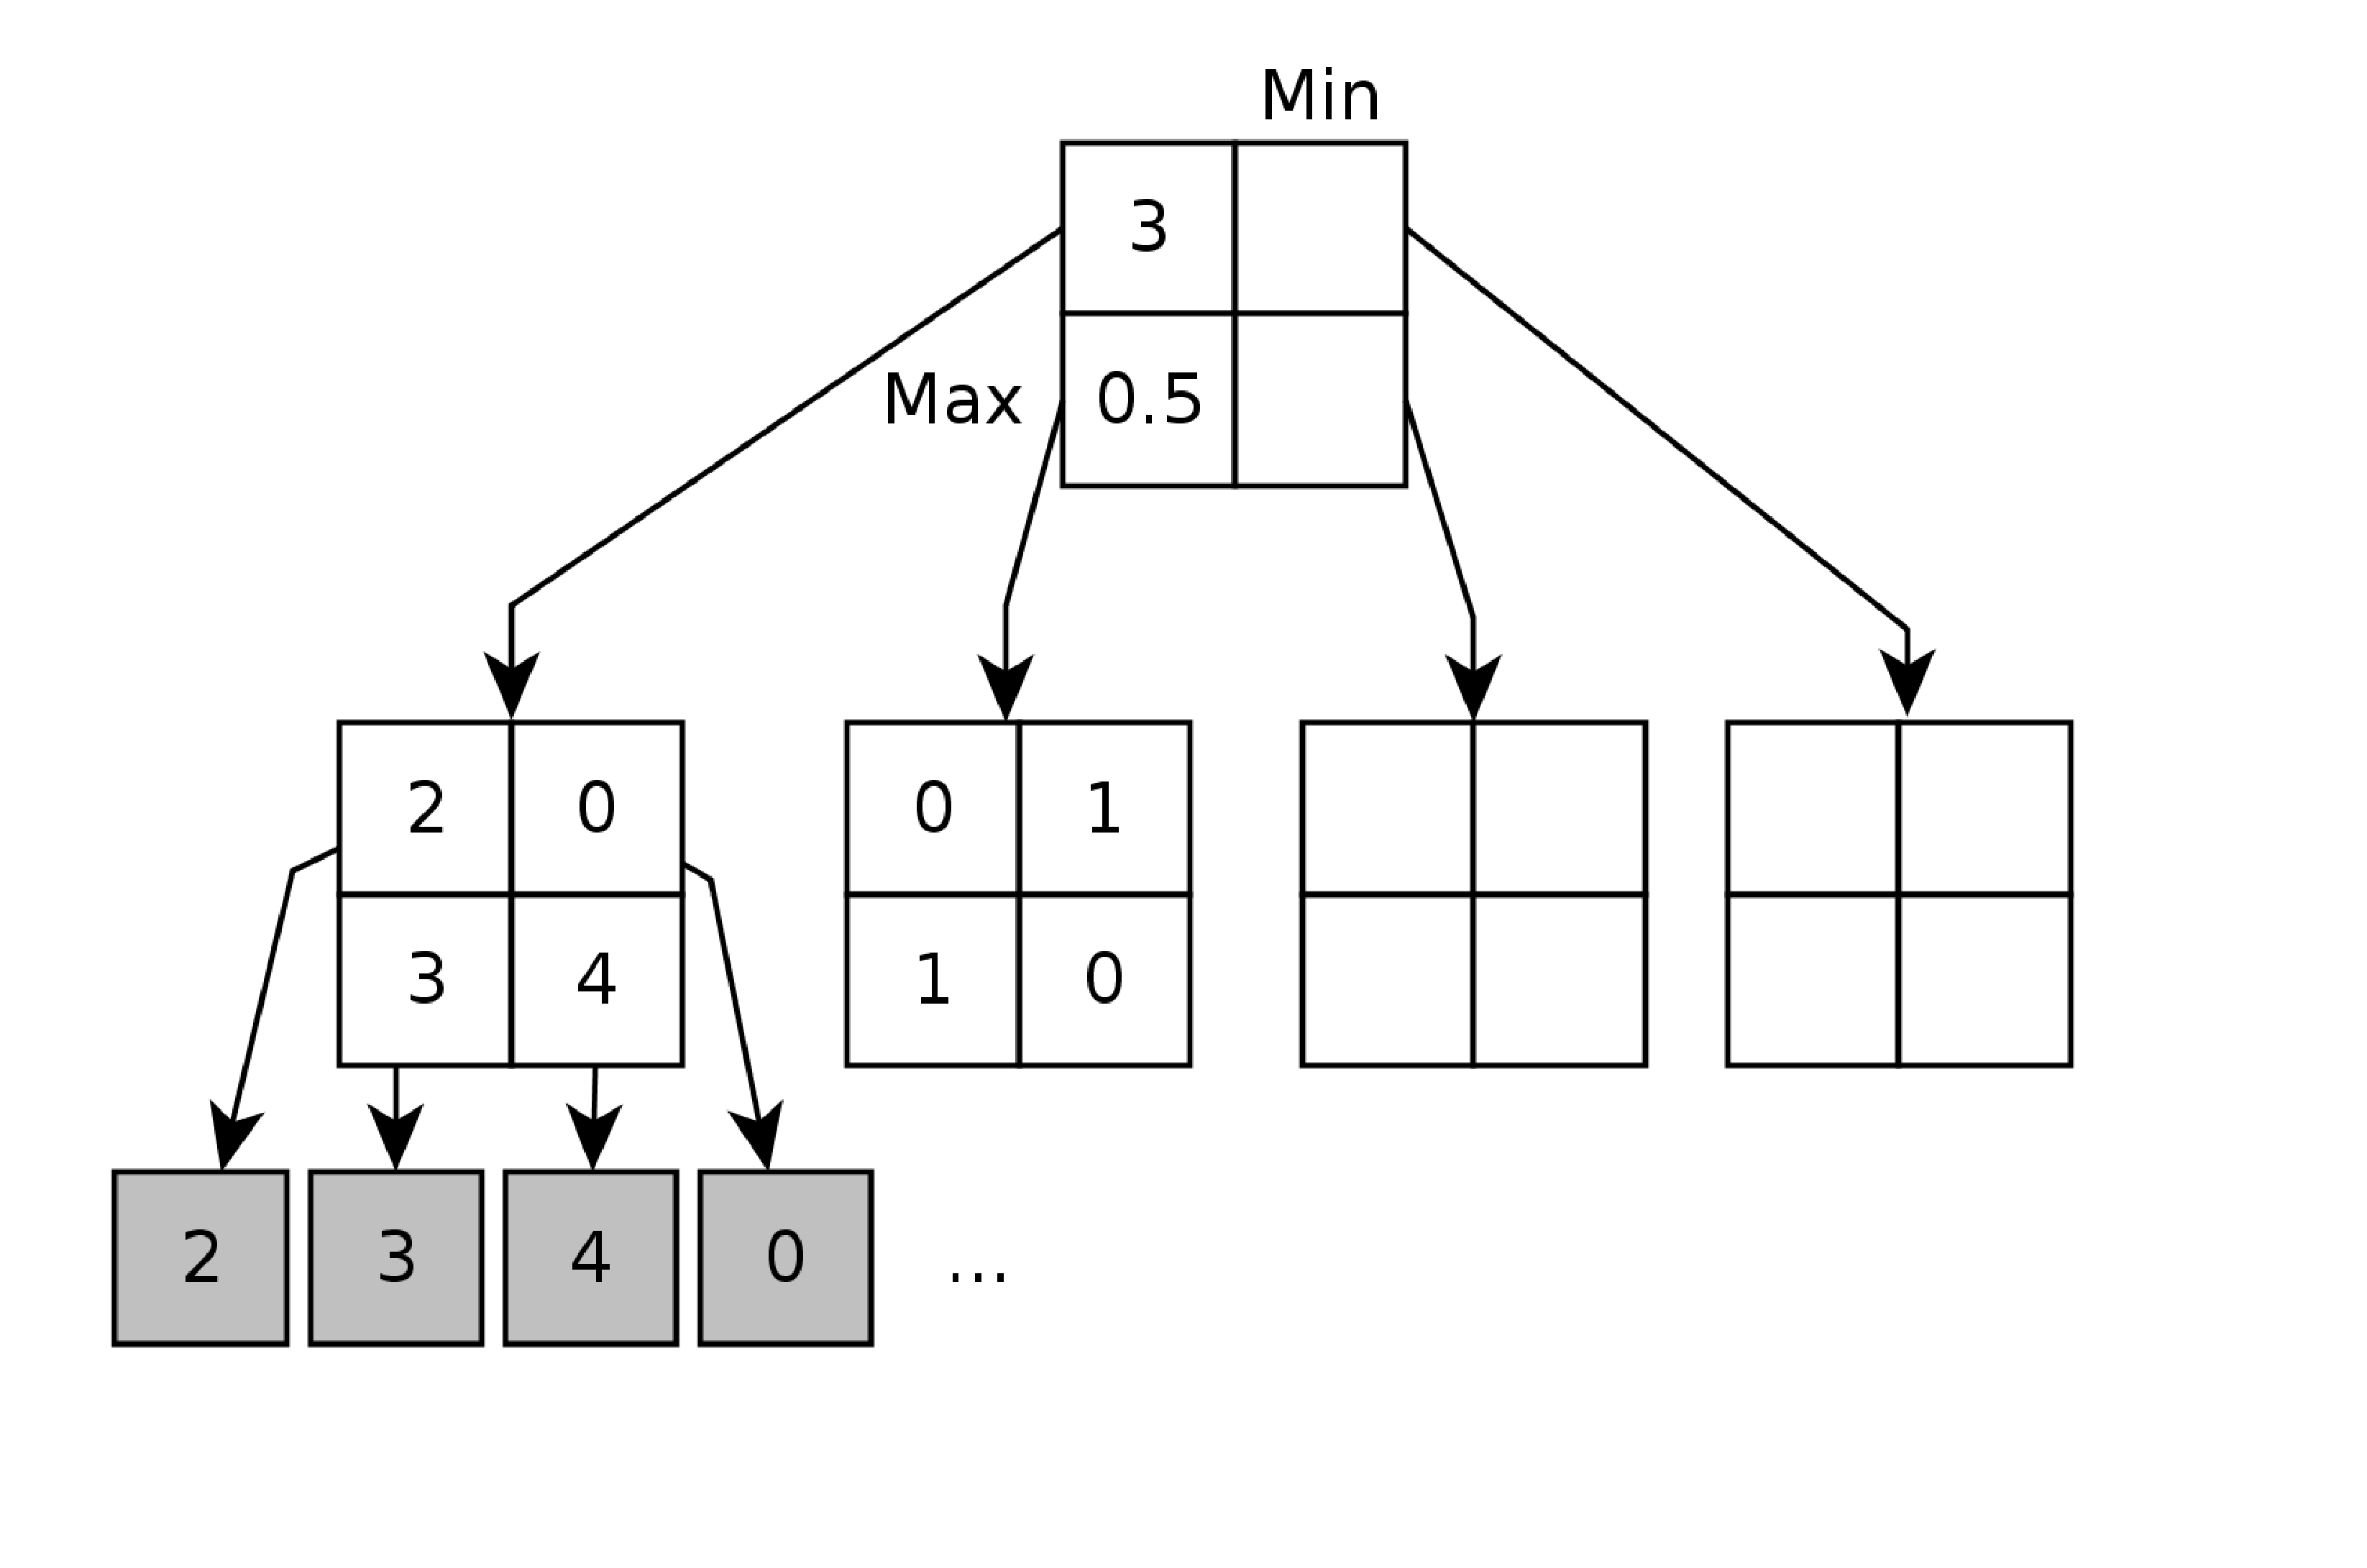
\includegraphics[width=6.0cm]{figures/tree}\\
\end{subfigure}
\caption{An examples of a two-player simultaneous game which has Matching Pennies as a subgame.
The dark squares are terminal states. The values shown are optimal values that could be obtained by backward induction.
{\small Note: the figure is taken from \cite{Lanctot13Goofspiel} and provided by Branislav Bosansky.}
\label{fig:example}}
\end{figure}

A {\it matrix game} is a single step simultaneous move game with action sets $\cA_1$ and $\cA_2$. 
Each entry in the matrix $A_{rc}$ where $(r,c) \in A_1 \times A_2$ corresponds to a payoff (to player 1) if row $r$ is chosen by player 1 and column $c$ by player 2. 
For example, in Matching Pennies, each player has two actions (heads or tails). The row player receives a payoff of 1 if both players choose the same action and 0 if they do not match. 
Two-player simultaneous move games are sometimes called {\it stacked matrix games} because at every state 
$s$ there is a joint action set $\cA_1(s) \times \cA_2(s)$ that either leads to a terminal state or to a subgame which 
is itself another stacked matrix game. 

A {\it behavioral strategy} for player $i$ is a mapping from states $s \in \cS$
to a probability distribution over the actions $\cA_i(s)$, denoted $\sigma_i(s)$. 
%Given a profile $\sigma = (\sigma_1, \sigma_2)$, define the probability of reaching a terminal state $z$ under $\sigma$ as 
%$\pi^\sigma(z) = \pi_1(z) \pi_2(z) \pi_c(z)$, where each $\pi_i(z)$ is a product of probabilities of the actions taken 
%by player $i$ along the path to $z$ ($c$ being chance's probabilities). 
Define $\Sigma_i$ to be the set of behavioral 
strategies for player $i$. A Nash equilibrium profile in this case is a pair of behavioral strategies optimizing
\begin{equation}\label{eq:ne}
V^* = \max_{\sigma_1 \in \Sigma_1} \min_{\sigma_2 \in \Sigma_2} \bE_{z \sim \sigma}[u_1(z)].
%   = \max_{\sigma_1 \in \Sigma_1} \min_{\sigma_2 \in \Sigma_2} \sum_{z \in Z} \pi^\sigma(z) u_1(z).
\end{equation}
In other words, none of the players can improve their utility by deviating unilaterally. 
For example, the Matching Pennies matrix game has a single state and the only equilibrium strategy is to mix equally between both actions, \ie play with a {\it mixed strategy} (distribution) of $(0.5, 0.5)$ giving an expected payoff of $V^* = 0.5$. 
If the strategies also optimize Equation \ref{eq:ne} in each subgame starting in an arbitrary state, the equilibrium strategy is termed subgame perfect.

In two-player constant-sum games a Nash equilibrium strategy is optimal in the minimax sense. It guarantees the payoff of at least $V^*$ against any opponent. Any 
non-equilibrium strategy has a best response, which will make it win less than $V^*$ in expectation. Moreover, subgame perfect NE strategy can earn more 
than $V^*$ against weak opponents. After the opponent makes a sub-optimal move, the strategy will never allow it to gain the loss back. 
The value $V^*$ is known as the minimax-optimal value of the game and is the same for every equilibrium profile by von Neumann's minimax theorem.

%A two-player simultaneous move game is a specific type of two-player imperfect information extensive-form 
%game. In imperfect information games, states are grouped into {\it information sets}: two states $s, s' \in I$ if the player 
%to act at $I$ cannot distinguish which of these states the game is currently in. Any simultaneous move game can be modeled 
%using an information set to represent a half-completed transition, \ie $\cT(s, a_1, ?)$ or $\cT(s, ?, a_2)$. 

An example of a simultaneous move game is depicted in Figure~\ref{fig:example}. 
The model described above is similar to a two-player finite horizon Markov Game~\cite{Littman94markovgames}.
The model can be easily extended to include chance events~\cite{Lanctot13Goofspiel}. 

\section{Simultaneous Move MCTS}
\label{sec:smmcts}

\newcommand{\SMMCTS}{{\sc SM-MCTS}}
\newcommand{\ExpReq}{{\sc ExpansionRequired}}
\newcommand{\Update}{{\sc Update}}
\newcommand{\Select}{{\sc Select}}
\newcommand{\Playout}{{\sc Playout}}
\newcommand{\Max}{\text{Max}}
\newcommand{\Min}{\text{Min}}


In this section, we present a generalized description of Monte Carlo Tree Search for simultaneous move games. This 
description is based on the one used in Tron~\cite{Perick12Comparison}. First, we describe the overall process. 
Each specific step (\Select, \Update, and final move selection) depends on the chosen variant described in the 
appropriate subsection. 

\begin{algorithm2e}[t!]
  \SMMCTS$($node $s$)\\                         \label{alg:function}
  \pushline
    \lIf{$s$ is a terminal state ($s \in \cZ$)}{\Return{$u_1(s)$}}
    \ElseIf{$s \in T$ {\bf and} \ExpReq$(s)$}{  \label{alg:expand}
      Choose a previously unselected $(a_1,a_2)$ \\
      $s' \gets \cT(s,a_1,a_2)$ \label{alg:choose-expand} \\
      Add $s'$ to $T$\\
      $u_1 \gets$ \Playout($s'$)\\
      $X_{s'} \gets X_{s'} + u_1$ \\
      $n_{s'} \gets n_{s'} + 1$  \\     \label{alg:increment2}
      \Update$(s, a_1, a_2, u_1)$\\                     \label{alg:update1}
      {\bf return} $u_1$\\
    }                                       
    $(a_1, a_2) \gets $  \Select$(s)$\\        \label{alg:select}
    $s' \gets \cT(s, a_1, a_2)$\\
    $u_1 \gets $ \SMMCTS($s'$)\\                \label{alg:reccall}
    \Update$(s, a_1, a_2, u_1)$ \\                      \label{alg:update2}
    {\bf return} $u_1$\\
  \popline
  \vspace{0.1cm}
  \caption{Simultaneous Move Monte Carlo Tree Search \label{alg:sm-mcts}}
\end{algorithm2e}


In Simultaneous Move MCTS (SM-MCTS), the main difference is that a joint action is selected. The convergence to an 
optimal strategy depends critically on the selection and update policies applied, which are not as straightforward 
as in purely sequential games. 
Algorithm~\ref{alg:sm-mcts} describes a single simulation of SM-MCTS. 
$T$ represents the MCTS tree in which each state is represented by one node. Every node $s$ maintains a 
cumulative reward sum over all simulations through it, $X_s$, and a visit count $n_s$, both initially set to 0. 
As with standard MCTS, when a state is visited these values are incremented on line \ref{alg:increment2}, and in the node 
updates on lines \ref{alg:update1} and \ref{alg:update2}. 
As seen in Figure~\ref{fig:example}, a matrix of references to the children is maintained at each state. 

At node $s$, the estimated values $\bar{X}_{s'}$ of the children nodes $s' = \cT(s,a_1,a_2)$ over all 
joint actions form an estimated payoff matrix for node $s$. 
The critical parts of the algorithm are the updates on lines \ref{alg:update1} and \ref{alg:update2}, and the selection 
on line \ref{alg:select}. Each variant below will describe a different way to select a joint action and update a node. 

In practice, there are several optimizations to the base algorithm that might be desirable.
If a game has a large branching factor, it may take many iterations for 
the expansion condition and consequence in lines \ref{alg:expand} to \ref{alg:choose-expand} to fill up the matrix before 
switching to a selection policy. 
The matrix can instead be filled such that at least one action has been taken from each row and one from each column before 
switching to the selection policy. 
Since most variants do not require values for each entry in the matrix, this could reduce the number of simulations before 
switching to $|\cA_1(s)| + |\cA_2(s)|$ from $|\cA_1(s)||\cA_2(s)|$. The use of progressive 
widening~\cite{Chaslot08Progressive} may also lead to deeper searches. 
In this paper, the implementation for experiments is based on the pseudo-code presented in Algorithm~\ref{alg:sm-mcts}.

\subsection{Decoupled UCT} 

In Decoupled UCT (DUCT), each player $i$ maintains for every state $s$ separate reward sums $X^i_{s,a}$ and 
visit counts $n^i_{s,a}$ for their own action set $a \in \cA_i(s)$. 
In essence, each player {\it decouples} the matrix in each state and applies UCB over the cumulative rewards for 
each of their own actions as if there was no joint dependency on these rewards.
When a joint action needs to be selected on line 
\ref{alg:select}, each player selects an action that maximizes the decoupled UCB value over their reward estimates 
independently:
\begin{equation}
\label{eq:duct}
a_i = \argmax_{a \in A_i(s)}{ \left\{ \bar{X}^i_{s,a} + C_i \sqrt{\frac{\ln n_s}{n_{s,a}}} \right\} }, 
  \mbox{ where } \bar{X}^i_{s,a} = \frac{X^i_{s,a}}{n_{s,a}}
\end{equation}
\noindent In DUCT, \Update~simply increments the decoupled values for each player $i$: $X^i_{s,a_i} \leftarrow X^i_{s,a_i} + u_i$,
and $n_{s,a_i} \leftarrow n_{s,a_i} + 1$. 

As an example, consider the game in Figure~\ref{fig:example}, with player set $\cN = \{\Max,\Min\}$, root node $s$,
and action sets $\cA_{\Max}(s) = \{t,b\}, \cA_{\Min}(s) = \{l,r\}$ representing top, bottom, left, and right. 
Suppose four simulations are run, and rewards received are $u_\Max = 3$ for $(t,l)$, $2$ for $(t,r)$, $1$ for $(b,l)$, 
and $0$ for $(b,r)$. The tree would contain exactly five states: $s$, and each child of $s$. On the fifth simulation, 
\Max~chooses among $t$ and $b$ and \Min~chooses among $r$ and $l$, both by using Equation~\ref{eq:duct}. 
In this case, $\bar{X}_{s,t}^\Max = (3 + 2) / 2 = 2.5$ and $\bar{X}_{s,b}^\Max = (1 + 0) / 2 = 0.5$. 
Supposing $v_{\max} = 4$, then $\bar{X}_{s,l}^\Min = (1 + 3) / 2 = 2$ and $\bar{X}^\Min_{s,r} = (2 + 4) / 2 = 3$. 

An enhancement to the UCT selection strategy can be made by replacing the parameter $C$ by an upper bound of the variance of 
the rewards. This is either $\frac{1}{4}$, which is an upper bound of the variance of a $\{0,1\}$-outcome Bernoulli
random variable, or an upper confidence bound computed using Equation~\ref{ucb1tuned}. 
This variant is referred to as UCB1-Tuned~\cite{Auer02Finite}. Then, an action is selected from parent 
node $s$ using:

\begin{equation}
\label{ucb1tuned}
a^* = \argmax_{a \in \cA(s)} \left\{ \bar{X}_{s,a} + \sqrt{\frac{\min(\frac{1}{4},\mathrm{Var}_{\mathit{UCB1}}(s,a)) \ln (n_{s})}{n_{s,a}}} \right\}, 
\end{equation}
\[
\mbox{Var}_{\mathit{UCB1}}(s,a)=\mbox{sv}^2_{s,a}+\sqrt{\frac{2 \ln (n_{s})}{n_{s,a}}},
\]
where $\mbox{sv}^2_{s,a}$ is the sample variance of the observed rewards for taking action $a$ from $s$. 
When UCB1-Tunded is used in the tree setting, we refer to it as the SM-MCTS variant {\it Decoupled UCB1-Tuned}, or DUCB1T for short.


\subsection{Exp3}

In Exp3~\cite{Exp3}, each player maintains an estimate of the sum of rewards, denoted $\hat{x}^i_{s,a}$, and visit 
counts $n^i_{s,a}$ for each of their own actions. 
Since these values and strategies are maintained separately for each player, 
Exp3 is decoupled in the same sense as DUCT. 

The joint action selected on line \ref{alg:select} is composed of actions independently selected for each player 
based on a sampling probability distribution composed for each player based on $\hat{x}^i_{s,a}$. 
The probability of sampling action $a_i$ is
\begin{equation}
\label{eq:exp3select}
\sigma^t_i(s,a_i) = \frac{(1-\gamma) \exp(\eta w^i_{s,a_i})}{\sum_{a_j \in \cA_i(s)} \exp(\eta w^i_{s,a_j})} + \frac{\gamma}{|\cA_i(s)|}, \mbox{ where }
\end{equation}
\[ \eta = \frac{\gamma}{|\cA_i(s)|}, \mbox{ and } w^i_{s,a} = \hat{x}^i_{s,a} - \max_{a' \in \cA_i(s)} \hat{x}^i_{s,a'}. \]

The update after selecting actions $(a_1,a_2)$ and obtaining a simulation result $(u_1,u_2)$ updates the visits count 
and adds to the corresponding reward sum estimates the reward divided by the probability that the action was played by the player using
\[n_{s,a_i} \leftarrow n_{s,a_i} + 1, ~~~ \hat{x}^i_{s,a_i} \leftarrow \hat{x}^i_{s,a_i} + \frac{u_i}{\sigma^t_i(s,a_i)}.\]
Dividing the value by the probability of selecting the corresponding action makes $\hat{x}^i_{s,a}$ estimate the sum of rewards over all 
iterations, not only the ones where $a_i$ was selected. 

The mixed strategy used by player $i$ after the simulations are done is given by the frequencies of visit counts of the actions, 
\[\sigma^{final}_i(s,a_i) = \frac{n_{s,a_i}}{\sum_{b_i\in A_i(s)} n_{s,b_i}}.\]
Previous work \cite{Teytaud11Upper} suggests first removing the samples caused by the exploration. This modification proved to be useful also in our experiments, so before computing the resulting final mixed strategy, we set
\begin{equation}
n_{s,a_i}' \leftarrow \max\left(0,n_{s,a_i} - \frac{\gamma}{|A_i(s)|}\sum_{b_i\in A_i(s)}n_{s,b_i}\right).
\end{equation}
For final move selection, a move is chosen by sampling according to a distribution that normalizes $n'_{s,a_i}$. 

\subsection{Regret Matching}

This variant applies regret matching \cite{Hart00} to the current estimated matrix game at each stage. 
Suppose iterations are numbered from $t \in \{ 1, 2, 3, \cdots \}$ and at each iteration and each node $s$ 
there is a mixed strategy $\sigma_i^t(s)$ used by each player $i$ for each node $s$ in the tree, initially set to 
uniform random: $\sigma^0_i(s,a) = 1 / |\cA(s)|$. 
Each player $i$ maintains a cumulative regret $r^i_s[a]$ for having played $\sigma_i^t(s)$ instead of $a \in \cA_i(s)$. 
In addition, a table for the average strategy is maintained per player as well $\bar{\sigma}^i_s[a]$. The values in 
both tables are initially set to 0. 
As in DUCT, the regret values $r^i_s[a_i]$ are maintained separately by each player.
However, the updates and specifically the reward uses a value that is a function of the joint action space. 

On iteration $t$, the selection policy (line \ref{alg:select} in Algorithm~\ref{alg:sm-mcts}) first builds 
the player's current strategies from the cumulative regret. Define $x^+ = \max(x,0)$,
\begin{equation}
\label{eq:rm}
\sigma^t_i(s,a) = \frac{r^i_s[a]}{R^+_{sum}} \mbox{ if } R^+_{sum} > 0 
\mbox{ oth. } \frac{1}{|\cA_i(s)|},  
\end{equation}
where $R^+_{sum} = \sum_{a \in \cA_i(s)}{r^{i,+}_s[a]}$. 
The main idea is to adjust the strategy by assigning higher weight proportionally to actions based on the regret of 
having not taken them over the long-term. 
To ensure exploration, an $\gamma$-on-policy sampling procedure similar to Equation~\ref{eq:exp3select} is used 
choosing action $a$ with probability $\gamma/|\cA(s)| + (1-\gamma) \sigma^t_i(s,a)$. 

The updates on line \ref{alg:update1} and \ref{alg:update2} add regret accumulated at the iteration to  
the regret tables $r^i_s$ and the average strategy $\bar{\sigma}^i_s[a]$. 
Suppose joint action $(a_1,a_2)$ is 
sampled from the selection policy and utility $u_i$ is returned from the recursive call on line~\ref{alg:reccall}. 
Label the current child $(i,j)$ estimate $\bar{X}_{s,i,j}$ and the $reward(i,j) = \bar{X}_{s,i,j}$ if 
$(i,j) \not= (a_1,a_2)$, or $u_i$ otherwise. The updates to the regret are:
\begin{eqnarray*}
\forall a_1' \in \cA_1(s),  r^1_s[a_1'] \leftarrow r^1_s[a_1'] + ( reward(a_1', a_2) - u_1 ),\\
\forall a_2' \in \cA_2(s),  r^2_s[a_2'] \leftarrow r^2_s[a_2'] + ( reward(a_1, a_2') - u_2 ),
\end{eqnarray*}
\noindent and average strategy updates are $\bar{\sigma}^i_s[a] \leftarrow \bar{\sigma}^i_s[a] + \sigma^t_i(s,a)$ 
for each player.

The final move for the root $s$ is chosen by sampling over the strategy obtained by 
normalizing the values in $\bar{\sigma}_s^i$. 

\subsection{Sequential UCT}



\section{Application to General Game-Playing}
\label{sec:appggp}

In this section, we discuss specific adaptations of SM-MCTS to general game playing.

In GGP, all utilities are non-negative, so without loss of generality, $v_{\min} = 0$. 
Also, games may not be constant-sum. In our implementation, we ensure that all payoffs 
are appropriately scaled to ensure that they are $k$-sum, with $k > 0$, by using 
a similar transformation previously used in Cadiaplayer~\cite{Finnsson12}:
\[ \text{\sc Scale}(u_1, u_2) = \left( \frac{u_1 - u_2 + k}{2k}, \frac{u_2 - u_1 + k}{2k} \right). \]

\subsection{Using N-Grams for Dynamic Playout Policies}

\subsection{Game Descriptions}

In this subsection, we describe nine simultaneous move games used to evaluate SM-MCTS in GGP. Some of these 
descriptions are teaken from~\cite[Appendix C]{Finnsson12}.

\textit{Battle} is played on an 8$\times$8 board. Each player has 20 disks. These disks can move one square or 
capture an opponent square next to them. Instead of a move, the player can choose to defend a square occupied by their 
piece. If an attacker attacks such a defended square, the attacker will be captured. The goal is to be the first player 
to capture 10 opponent disks. 

\textit{Bidding Tic-Tac-Toe} is a variation of normal Tic-Tac-Toe where there is a bidding round between 
normal play that decides who gets to place a marker on the board. Each player begins with three coins, and the 
\textsc{x} player has an additional tiebreaker token. When a player wins a bidding round, allowing that player to 
place a marker, the coins used to bid are given to the opponent. The tiebreaker token can optionally be used to break 
ties, and if so, the tiebreaker token is also given to the opponent. The winning conditions are the same as 
standard Tic-Tac-Toe. 

\textit{Chinook} is a variant of \textit{Breakthrough} where two independent games are played simultaneously. 
One game on the white squares and another one on the black squares. Black and White move their pieces simultaneously 
like Checkers pawns. As in Breakthrough, the first player that reaches the opposite side of the board wins the game. 

\textit{Goofspiel}$(N)$ is a card game where each player gets $N$ cards marked 1-$N$, and there is a central pile, 
shuffled and face down called the point-card deck (also 1-$N$). Every turn, the top card of this point card deck flips, 
it is called the {\it upcard}. Then, players choose a {\it bid} card from their hand and reveal it simultaneously. 
The player with the higher bid card obtains a number of points equal to the value of the upcard. The bid cards and 
upcard are then discarded and a new round starts. At the end of $N$ rounds, the player with the highest number of 
points wins. If the number of points are tied, the game ends in a draw. The standard game of Goofspiel has 
$N = 13$. In this paper, we assume that the point cards have a fixed order. 

In \textit{Runners} each turn both players decide how many steps they want to move forward or backward. The aim 
is to reach the goal location before the opponent does.

\textit{Oshi-Zumo}$(N,K,M)$ is a wrestling simulation game played on a discrete single-dimensional grid with 
$2K+1$ positions, where each player starts with $N$ coins~\cite{Buro03OshiZumo}. A wrestler token begins in the middle 
position. Every turn, 
each player bids $b \ge M$ coins. The coins bid are then discarded and the player bidding the most coins pushes the 
wrestler one position closer to the goal for that player. 

\textit{Pawn Whopping} is a simultaneous move version of Breakthrough, played on an 8 $\times$ 8 board. Each player has 
16 pawns starting on one side of the board and the goal is to move one of their pieces to the other side of the board. 
Pawns can capture diagonally and only move forward one cell straight or diagonally.
If opposing pawns try to capture each other or move to the same square, no change is made. 
Pawn Whopping has slightly different movement and is simultaneous.

\textit{Racetrack Corridor} is bla bla...

\textit{Tron} is a two-player game played on discrete two-dimensional grid possibly obstructed by walls. At each
step in Tron both players move to adjacent cells, and a wall is placed in the cells that the player started on that turn. 
The game is won if the opponent crashes into a wall or moves off the board. If both players crash at the same turn 
into a wall, the game ends in a draw.

\section{Empirical Evaluation}
\label{sec:exp}


\section{Conclusion and Future Work}
\label{sec:conc}


% An example of a floating figure using the graphicx package.
% Note that \label must occur AFTER (or within) \caption.
% For figures, \caption should occur after the \includegraphics.
% Note that IEEEtran v1.7 and later has special internal code that
% is designed to preserve the operation of \label within \caption
% even when the captionsoff option is in effect. However, because
% of issues like this, it may be the safest practice to put all your
% \label just after \caption rather than within \caption{}.
%
% Reminder: the "draftcls" or "draftclsnofoot", not "draft", class
% option should be used if it is desired that the figures are to be
% displayed while in draft mode.
%
%\begin{figure}[!t]
%\centering
%\includegraphics[width=2.5in]{myfigure}
% where an .eps filename suffix will be assumed under latex, 
% and a .pdf suffix will be assumed for pdflatex; or what has been declared
% via \DeclareGraphicsExtensions.
%\caption{Simulation Results}
%\label{fig_sim}
%\end{figure}

% Note that IEEE typically puts floats only at the top, even when this
% results in a large percentage of a column being occupied by floats.


% An example of a double column floating figure using two subfigures.
% (The subfig.sty package must be loaded for this to work.)
% The subfigure \label commands are set within each subfloat command, the
% \label for the overall figure must come after \caption.
% \hfil must be used as a separator to get equal spacing.
% The subfigure.sty package works much the same way, except \subfigure is
% used instead of \subfloat.
%
%\begin{figure*}[!t]
%\centerline{\subfloat[Case I]\includegraphics[width=2.5in]{subfigcase1}%
%\label{fig_first_case}}
%\hfil
%\subfloat[Case II]{\includegraphics[width=2.5in]{subfigcase2}%
%\label{fig_second_case}}}
%\caption{Simulation results}
%\label{fig_sim}
%\end{figure*}
%
% Note that often IEEE papers with subfigures do not employ subfigure
% captions (using the optional argument to \subfloat), but instead will
% reference/describe all of them (a), (b), etc., within the main caption.


% An example of a floating table. Note that, for IEEE style tables, the 
% \caption command should come BEFORE the table. Table text will default to
% \footnotesize as IEEE normally uses this smaller font for tables.
% The \label must come after \caption as always.
%
%\begin{table}[!t]
%% increase table row spacing, adjust to taste
%\renewcommand{\arraystretch}{1.3}
% if using array.sty, it might be a good idea to tweak the value of
% \extrarowheight as needed to properly center the text within the cells
%\caption{An Example of a Table}
%\label{table_example}
%\centering
%% Some packages, such as MDW tools, offer better commands for making tables
%% than the plain LaTeX2e tabular which is used here.
%\begin{tabular}{|c||c|}
%\hline
%One & Two\\
%\hline
%Three & Four\\
%\hline
%\end{tabular}
%\end{table}


% Note that IEEE does not put floats in the very first column - or typically
% anywhere on the first page for that matter. Also, in-text middle ("here")
% positioning is not used. Most IEEE journals/conferences use top floats
% exclusively. Note that, LaTeX2e, unlike IEEE journals/conferences, places
% footnotes above bottom floats. This can be corrected via the \fnbelowfloat
% command of the stfloats package.


% conference papers do not normally have an appendix


% use section* for acknowledgement
%\section*{Acknowledgment}

% trigger a \newpage just before the given reference
% number - used to balance the columns on the last page
% adjust value as needed - may need to be readjusted if
% the document is modified later
%\IEEEtriggeratref{8}
% The "triggered" command can be changed if desired:
%\IEEEtriggercmd{\enlargethispage{-5in}}

% references section

% can use a bibliography generated by BibTeX as a .bbl file
% BibTeX documentation can be easily obtained at:
% http://www.ctan.org/tex-archive/biblio/bibtex/contrib/doc/
% The IEEEtran BibTeX style support page is at:
% http://www.michaelshell.org/tex/ieeetran/bibtex/
\bibliographystyle{IEEEtran}
% argument is your BibTeX string definitions and bibliography database(s)
%\bibliography{IEEEabrv,../bib/paper}
\bibliography{smmcts-ggp}
%
% <OR> manually copy in the resultant .bbl file
% set second argument of \begin to the number of references
% (used to reserve space for the reference number labels box)
%\begin{thebibliography}{1}
%\bibitem{IEEEhowto:kopka}
%H.~Kopka and P.~W. Daly, \emph{A Guide to \LaTeX}, 3rd~ed.\hskip 1em plus
%  0.5em minus 0.4em\relax Harlow, England: Addison-Wesley, 1999.
%\end{thebibliography}


% that's all folks
\end{document}


